\chapter{Basic components}
\section{Operational amplifier}

The first task is to implement an operational amplifier. The schematics of the differential stage and bias circuit of the OA are provided. The implemented amplifier is to be found in the file (\texttt{OpAmp}). The simulation results given on figure \ref{fig:opAmpSimulation} are obtained in Cadence with the following testbench (table \ref{table:opAmpTestbench}): 

\begin{table}[!h]
	\centering
	\begin{tabular}{|l|l|l|}
		\hline
		Name & Type & Value \\
		\hline
		$V_{dd}$ & constant & 1.2V \\
		$V_{ref}$, $V_{bias}$, $V_{-}$ & constant & 600mV \\
		$V_{+}$ (In) & pulse & AC=500mV, DC=0V, f=1MHz \\
		\hline
	\end{tabular}
	\label{table:opAmpTestbench}
	\caption{Operational amplifier testbench}
\end{table}

As expected, the operational amplifier is driven in a saturated operating regime and behaves as a comparator.

\begin{figure}[h]
	\centering
	\includegraphics[scale=0.65]{images/BasicComponents/Task1opAmpSimulation.png}
	\label{fig:opAmpSimulation}
	\caption{Operational amplifier simulation}
\end{figure} 

\section{Clock generator}

The second task consists in implementing a clock generator (\texttt{clkGen}) in Verilog. The Verilog code is provided. The results of the simulation in ModelSim are given on figure \ref{fig:clkGenSimulation}.

\begin{figure}[h]
	\centering
	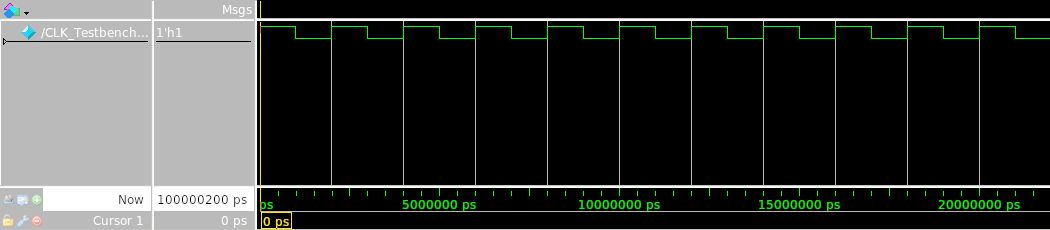
\includegraphics[scale=0.6]{images/BasicComponents/Task2ClkGenSimulation.png}
	\label{fig:clkGenSimulation}
	\caption{Clock generator simulation}
\end{figure}

For more configurability, an additional parameter \texttt{FKHZ} is introduced, which corresponds to the desired frequency in kHz.